% Part A. Included from results.tex with % Part A. Included from results.tex with % Part A. Included from results.tex with % Part A. Included from results.tex with \input{sections/partA_results}.
\subsection{Speed of Part A}
Part A was made faster without changing its output (banded solver, vectorised median filter,
channels in parallel threads). For the \SI{4.7}{\hour} recording it took \SI{1.71}{\second}
before and \SI{0.62}{\second} after on a MacBook, and about \SI{3.5}{\second} before and
\SI{2.0}{\second} after on a Windows laptop. Over all recordings compared on the MacBook it was
2.7 times faster.

\subsection{Noise level and threshold}
\label{sec:threshold-results}
\paragraph{Noise level.}
For the 28 recordings, the noise level $\sigma$ of \texttt{adc2} ranges from 0.51 to 4.03 counts
with a median of 1.32 counts (Figure~\ref{fig:sigma-pieces}, left), so the detection threshold
$10\sigma$ is measured separately for each recording. On the Big pieces recording, the median
and Savitzky--Golay filters lower $\sigma$ of \texttt{adc2} only slightly, from 1.09 to 1.03
counts, and the 20 tallest peaks keep a median of 96\,\% of their height (minimum 59\,\%).

\paragraph{Piece count and the threshold.}
To test how much the threshold matters, $k$ was varied from 5 to 30 with the same value for
all 28 recordings (Table~\ref{tab:k-sweep}, Figure~\ref{fig:sigma-pieces}, right). The number
of pieces depends strongly on $k$: at $k = 5$, noise peaks inflate the count, and between
$k = 8$ and $k = 30$ it grows slowly while the number of dyed pieces keeps rising. How the
threshold changes the estimated amount is treated with the amount of tissue.

\begin{table}[ht]
  \centering
  \caption{Pieces found in all 28 recordings, same settings for all recordings, threshold
  $k\sigma$ varied.}
  \label{tab:k-sweep}
  \begin{tabular}{rrr}
    \toprule
    $k$ & Pieces & Dyed pieces \\
    \midrule
    5  & 2142 & 318  \\
    8  & 954  & 557  \\
    10 & 977  & 645  \\
    15 & 1149 & 850  \\
    20 & 1207 & 953  \\
    30 & 1274 & 1066 \\
    \bottomrule
  \end{tabular}
\end{table}

\begin{figure}[ht]
  \centering
  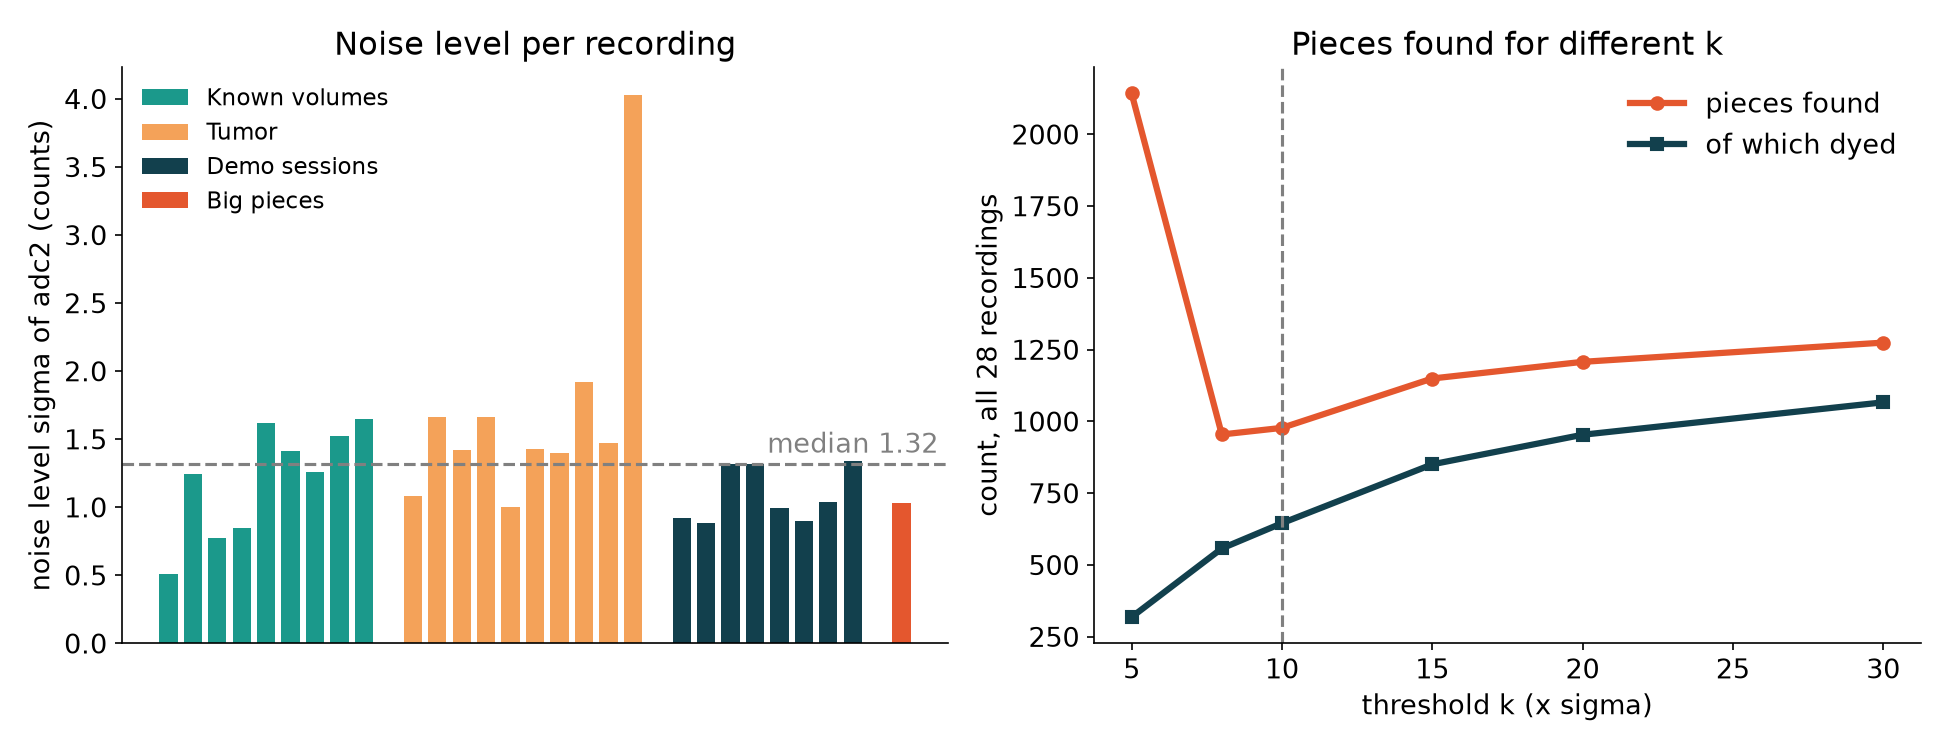
\includegraphics[width=\linewidth]{figures/partA_sigma_pieces.png}
  \caption{Left: noise level $\sigma$ of \texttt{adc2} for each of the 28 recordings.
  Right: number of pieces and of dyed pieces over all 28 recordings for different $k$.}
  \label{fig:sigma-pieces}
\end{figure}

\paragraph{One noise level for all recordings.}
Replacing the per-recording $\sigma$ by one common value (the median, 1.32 counts for
\texttt{adc2}) with $k = 10$ changes the number of pieces in 23 of the 28 recordings; for the
\SI{4.7}{\hour} recording it rises from 83 to 232. The common value was taken from these
recordings, so this is not an independent test.

\paragraph{Pieces at the edges of a recording.}
Only 10 of the 977 pieces (1\,\%) start within \SI{5}{\second} of the start or end within
\SI{5}{\second} of the end of a recording.
.
\subsection{Speed of Part A}
Part A was made faster without changing its output (banded solver, vectorised median filter,
channels in parallel threads). For the \SI{4.7}{\hour} recording it took \SI{1.71}{\second}
before and \SI{0.62}{\second} after on a MacBook, and about \SI{3.5}{\second} before and
\SI{2.0}{\second} after on a Windows laptop. Over all recordings compared on the MacBook it was
2.7 times faster.

\subsection{Noise level and threshold}
\label{sec:threshold-results}
\paragraph{Noise level.}
For the 28 recordings, the noise level $\sigma$ of \texttt{adc2} ranges from 0.51 to 4.03 counts
with a median of 1.32 counts (Figure~\ref{fig:sigma-pieces}, left), so the detection threshold
$10\sigma$ is measured separately for each recording. On the Big pieces recording, the median
and Savitzky--Golay filters lower $\sigma$ of \texttt{adc2} only slightly, from 1.09 to 1.03
counts, and the 20 tallest peaks keep a median of 96\,\% of their height (minimum 59\,\%).

\paragraph{Piece count and the threshold.}
To test how much the threshold matters, $k$ was varied from 5 to 30 with the same value for
all 28 recordings (Table~\ref{tab:k-sweep}, Figure~\ref{fig:sigma-pieces}, right). The number
of pieces depends strongly on $k$: at $k = 5$, noise peaks inflate the count, and between
$k = 8$ and $k = 30$ it grows slowly while the number of dyed pieces keeps rising. How the
threshold changes the estimated amount is treated with the amount of tissue.

\begin{table}[ht]
  \centering
  \caption{Pieces found in all 28 recordings, same settings for all recordings, threshold
  $k\sigma$ varied.}
  \label{tab:k-sweep}
  \begin{tabular}{rrr}
    \toprule
    $k$ & Pieces & Dyed pieces \\
    \midrule
    5  & 2142 & 318  \\
    8  & 954  & 557  \\
    10 & 977  & 645  \\
    15 & 1149 & 850  \\
    20 & 1207 & 953  \\
    30 & 1274 & 1066 \\
    \bottomrule
  \end{tabular}
\end{table}

\begin{figure}[ht]
  \centering
  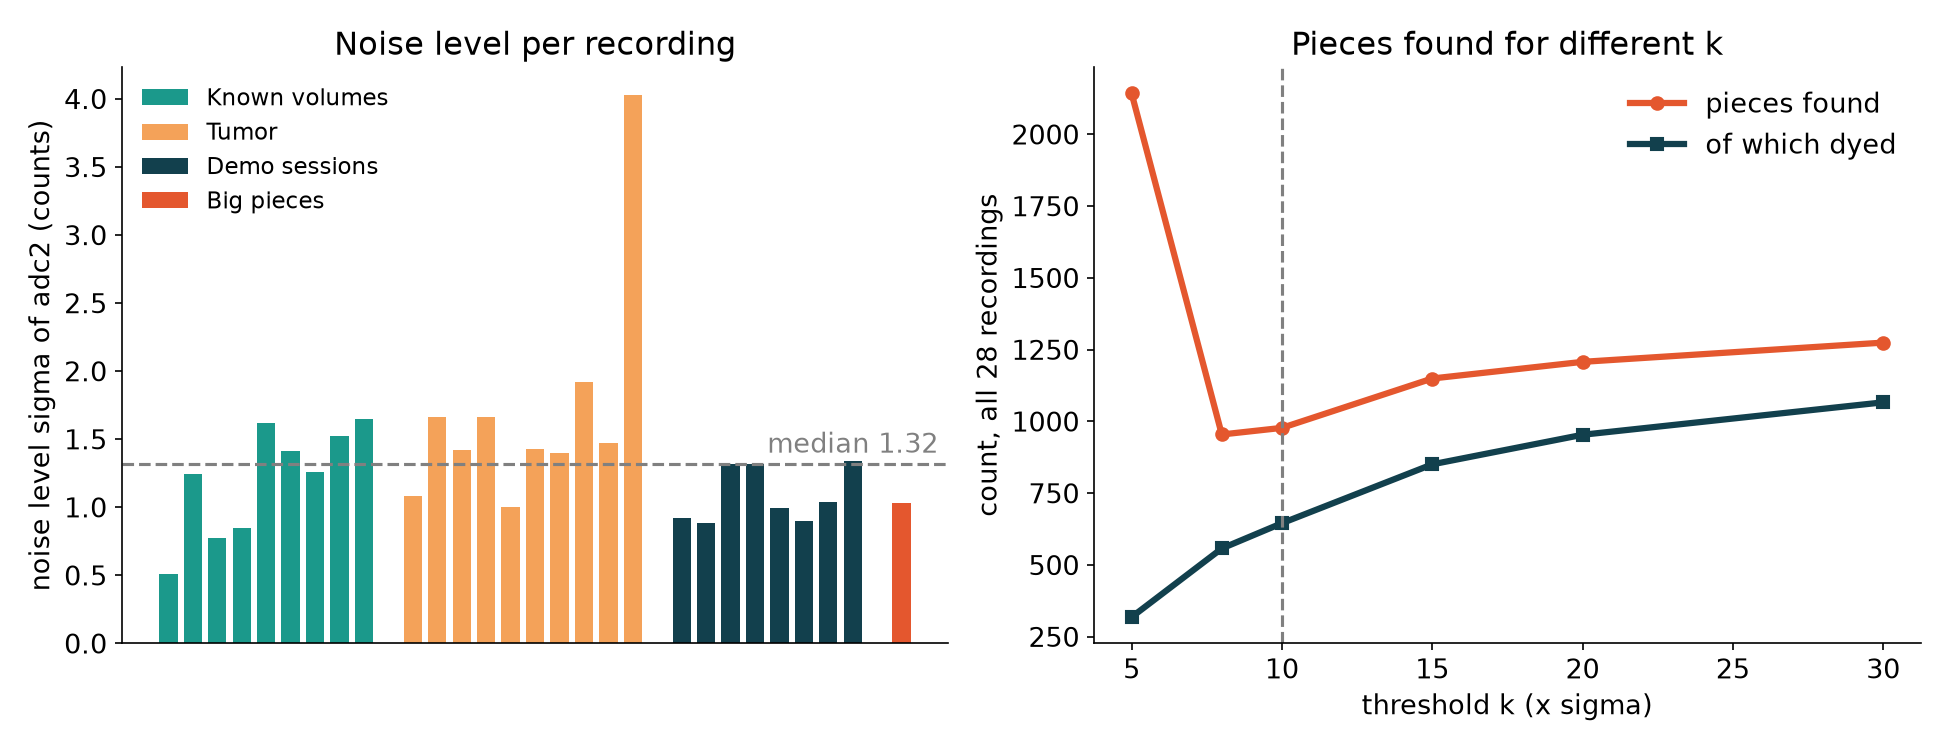
\includegraphics[width=\linewidth]{figures/partA_sigma_pieces.png}
  \caption{Left: noise level $\sigma$ of \texttt{adc2} for each of the 28 recordings.
  Right: number of pieces and of dyed pieces over all 28 recordings for different $k$.}
  \label{fig:sigma-pieces}
\end{figure}

\paragraph{One noise level for all recordings.}
Replacing the per-recording $\sigma$ by one common value (the median, 1.32 counts for
\texttt{adc2}) with $k = 10$ changes the number of pieces in 23 of the 28 recordings; for the
\SI{4.7}{\hour} recording it rises from 83 to 232. The common value was taken from these
recordings, so this is not an independent test.

\paragraph{Pieces at the edges of a recording.}
Only 10 of the 977 pieces (1\,\%) start within \SI{5}{\second} of the start or end within
\SI{5}{\second} of the end of a recording.
.
\subsection{Speed of Part A}
Part A was made faster without changing its output (banded solver, vectorised median filter,
channels in parallel threads). For the \SI{4.7}{\hour} recording it took \SI{1.71}{\second}
before and \SI{0.62}{\second} after on a MacBook, and about \SI{3.5}{\second} before and
\SI{2.0}{\second} after on a Windows laptop. Over all recordings compared on the MacBook it was
2.7 times faster.

\subsection{Noise level and threshold}
\label{sec:threshold-results}
\paragraph{Noise level.}
For the 28 recordings, the noise level $\sigma$ of \texttt{adc2} ranges from 0.51 to 4.03 counts
with a median of 1.32 counts (Figure~\ref{fig:sigma-pieces}, left), so the detection threshold
$10\sigma$ is measured separately for each recording. On the Big pieces recording, the median
and Savitzky--Golay filters lower $\sigma$ of \texttt{adc2} only slightly, from 1.09 to 1.03
counts, and the 20 tallest peaks keep a median of 96\,\% of their height (minimum 59\,\%).

\paragraph{Piece count and the threshold.}
To test how much the threshold matters, $k$ was varied from 5 to 30 with the same value for
all 28 recordings (Table~\ref{tab:k-sweep}, Figure~\ref{fig:sigma-pieces}, right). The number
of pieces depends strongly on $k$: at $k = 5$, noise peaks inflate the count, and between
$k = 8$ and $k = 30$ it grows slowly while the number of dyed pieces keeps rising. How the
threshold changes the estimated amount is treated with the amount of tissue.

\begin{table}[ht]
  \centering
  \caption{Pieces found in all 28 recordings, same settings for all recordings, threshold
  $k\sigma$ varied.}
  \label{tab:k-sweep}
  \begin{tabular}{rrr}
    \toprule
    $k$ & Pieces & Dyed pieces \\
    \midrule
    5  & 2142 & 318  \\
    8  & 954  & 557  \\
    10 & 977  & 645  \\
    15 & 1149 & 850  \\
    20 & 1207 & 953  \\
    30 & 1274 & 1066 \\
    \bottomrule
  \end{tabular}
\end{table}

\begin{figure}[ht]
  \centering
  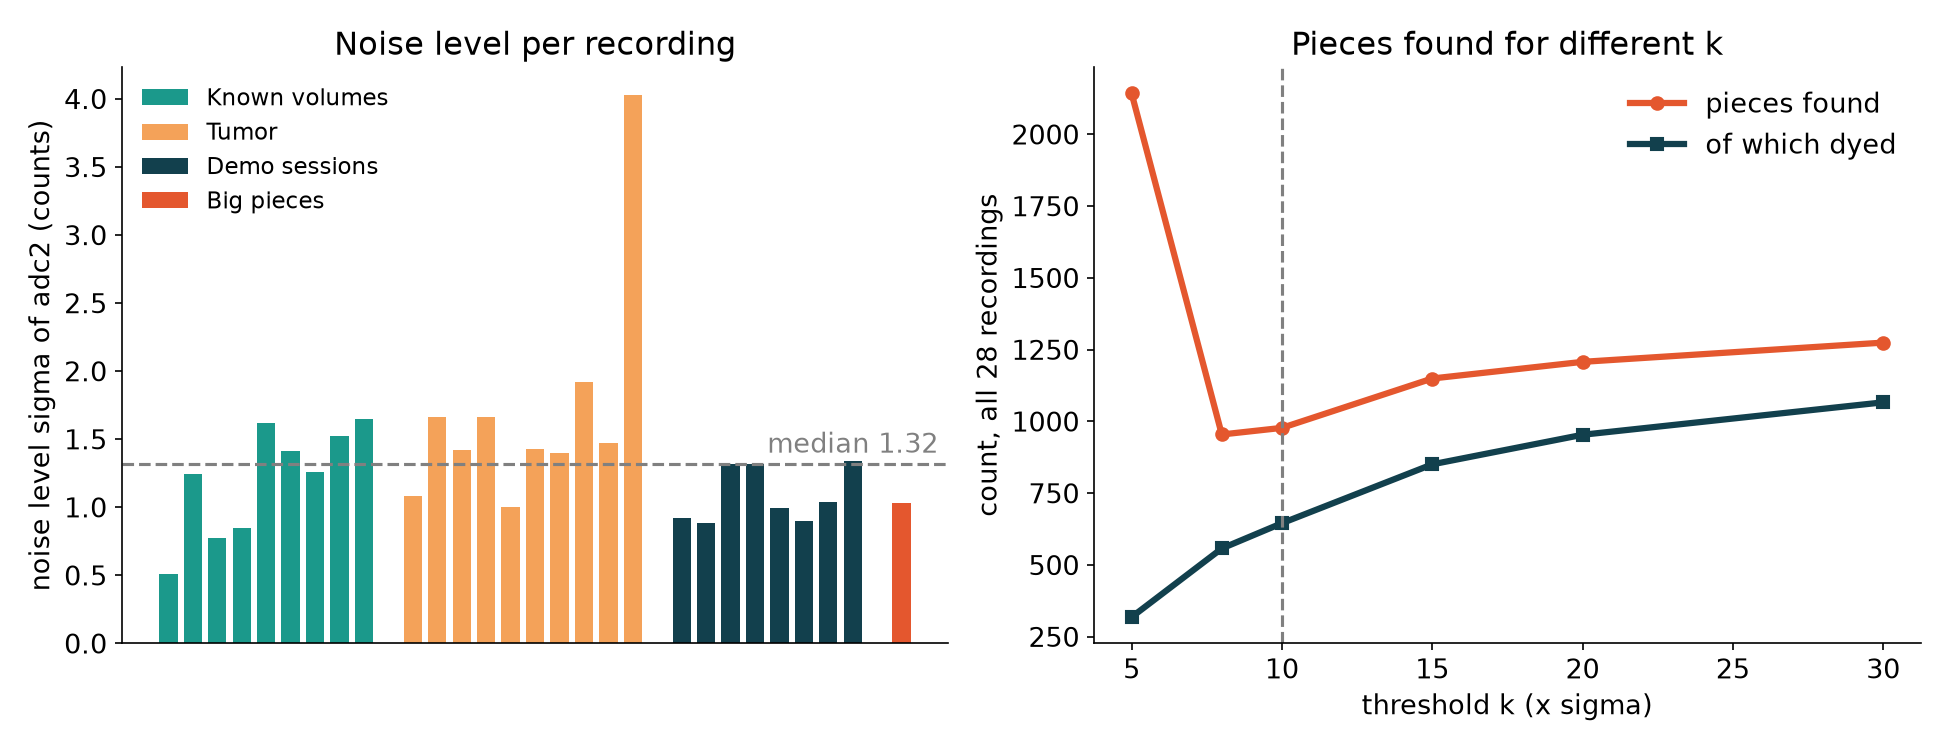
\includegraphics[width=\linewidth]{figures/partA_sigma_pieces.png}
  \caption{Left: noise level $\sigma$ of \texttt{adc2} for each of the 28 recordings.
  Right: number of pieces and of dyed pieces over all 28 recordings for different $k$.}
  \label{fig:sigma-pieces}
\end{figure}

\paragraph{One noise level for all recordings.}
Replacing the per-recording $\sigma$ by one common value (the median, 1.32 counts for
\texttt{adc2}) with $k = 10$ changes the number of pieces in 23 of the 28 recordings; for the
\SI{4.7}{\hour} recording it rises from 83 to 232. The common value was taken from these
recordings, so this is not an independent test.

\paragraph{Pieces at the edges of a recording.}
Only 10 of the 977 pieces (1\,\%) start within \SI{5}{\second} of the start or end within
\SI{5}{\second} of the end of a recording.
.
\subsection{Speed of Part A}
Part A was made faster without changing its output (banded solver, vectorised median filter,
channels in parallel threads). For the \SI{4.7}{\hour} recording it took \SI{1.71}{\second}
before and \SI{0.62}{\second} after on a MacBook, and about \SI{3.5}{\second} before and
\SI{2.0}{\second} after on a Windows laptop. Over all recordings compared on the MacBook it was
2.7 times faster.

\subsection{Noise level and threshold}
\label{sec:threshold-results}
\paragraph{Noise level.}
For the 28 recordings, the noise level $\sigma$ of \texttt{adc2} ranges from 0.51 to 4.03 counts
with a median of 1.32 counts (Figure~\ref{fig:sigma-pieces}, left), so the detection threshold
$10\sigma$ is measured separately for each recording. On the Big pieces recording, the median
and Savitzky--Golay filters lower $\sigma$ of \texttt{adc2} only slightly, from 1.09 to 1.03
counts, and the 20 tallest peaks keep a median of 96\,\% of their height (minimum 59\,\%).

\paragraph{Piece count and the threshold.}
To test how much the threshold matters, $k$ was varied from 5 to 30 with the same value for
all 28 recordings (Table~\ref{tab:k-sweep}, Figure~\ref{fig:sigma-pieces}, right). The number
of pieces depends strongly on $k$: at $k = 5$, noise peaks inflate the count, and between
$k = 8$ and $k = 30$ it grows slowly while the number of dyed pieces keeps rising. How the
threshold changes the estimated amount is treated with the amount of tissue.

\begin{table}[ht]
  \centering
  \caption{Pieces found in all 28 recordings, same settings for all recordings, threshold
  $k\sigma$ varied.}
  \label{tab:k-sweep}
  \begin{tabular}{rrr}
    \toprule
    $k$ & Pieces & Dyed pieces \\
    \midrule
    5  & 2142 & 318  \\
    8  & 954  & 557  \\
    10 & 977  & 645  \\
    15 & 1149 & 850  \\
    20 & 1207 & 953  \\
    30 & 1274 & 1066 \\
    \bottomrule
  \end{tabular}
\end{table}

\begin{figure}[ht]
  \centering
  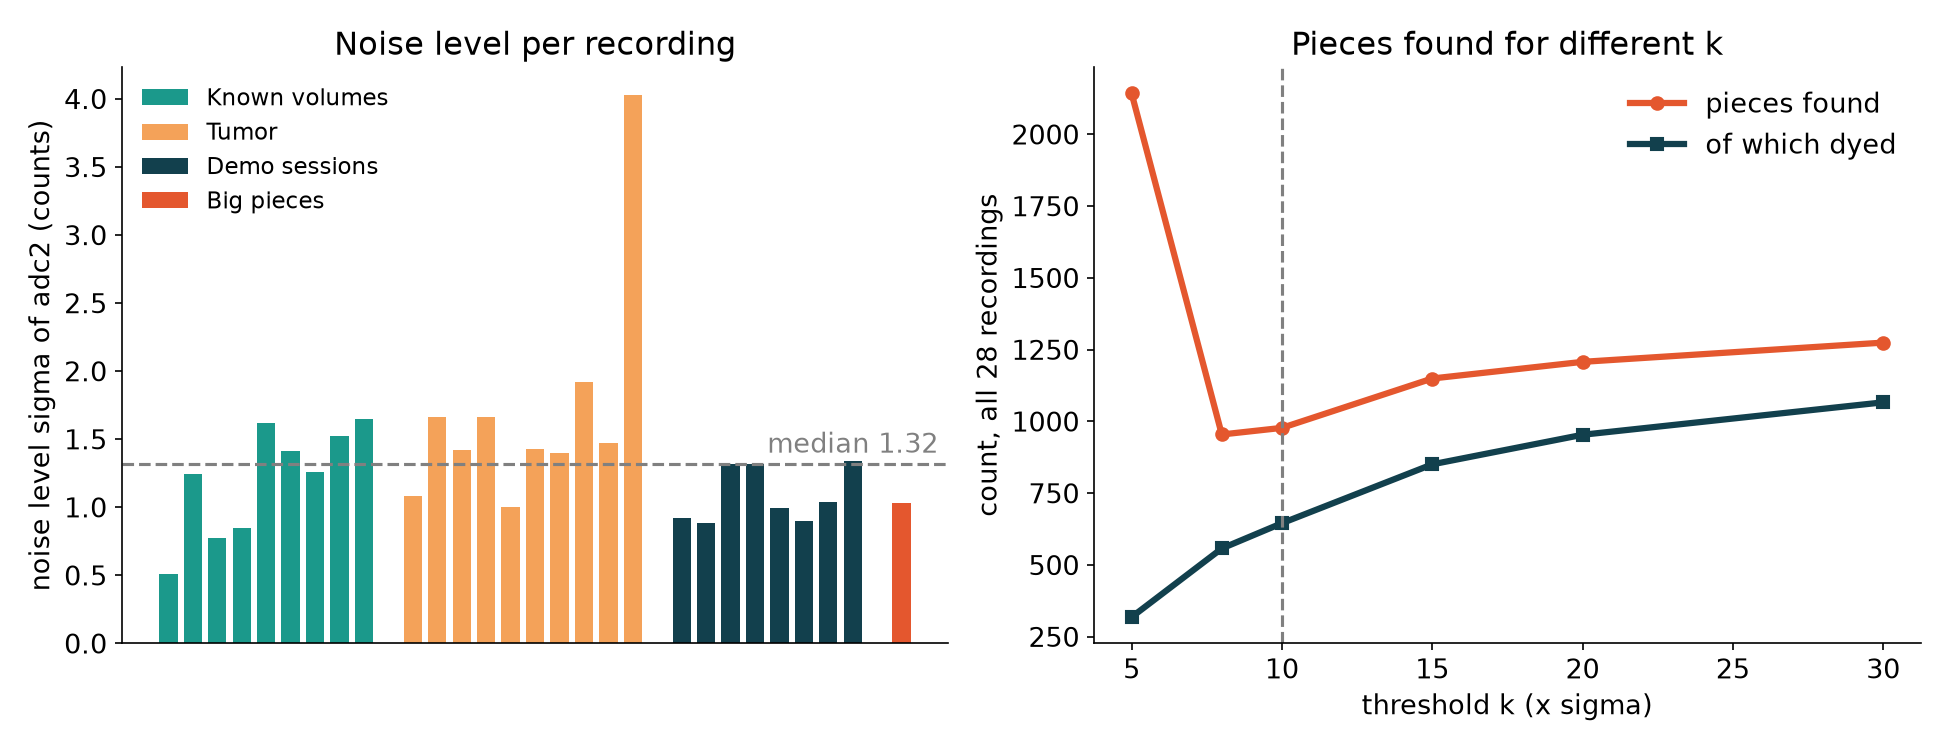
\includegraphics[width=\linewidth]{figures/partA_sigma_pieces.png}
  \caption{Left: noise level $\sigma$ of \texttt{adc2} for each of the 28 recordings.
  Right: number of pieces and of dyed pieces over all 28 recordings for different $k$.}
  \label{fig:sigma-pieces}
\end{figure}

\paragraph{One noise level for all recordings.}
Replacing the per-recording $\sigma$ by one common value (the median, 1.32 counts for
\texttt{adc2}) with $k = 10$ changes the number of pieces in 23 of the 28 recordings; for the
\SI{4.7}{\hour} recording it rises from 83 to 232. The common value was taken from these
recordings, so this is not an independent test.

\paragraph{Pieces at the edges of a recording.}
Only 10 of the 977 pieces (1\,\%) start within \SI{5}{\second} of the start or end within
\SI{5}{\second} of the end of a recording.
